Recall that an \define{environment diagram} keeps track of all the variables that have been defined and the values they are bound to.
However, values are not necessarily only integers and strings. Environment diagrams can model more complex programs that utilize higher order functions.

\setlength{\parindent}{0cm}
\begin{minipage}{0.4\textwidth}
\begin{lstlisting}[linewidth=\textwidth]
def add_num(x):
    return lambda y: x + y

add_two = add_num(2)
add_two(3)
\end{lstlisting}
\end{minipage}
\begin{minipage}{0.6\textwidth}
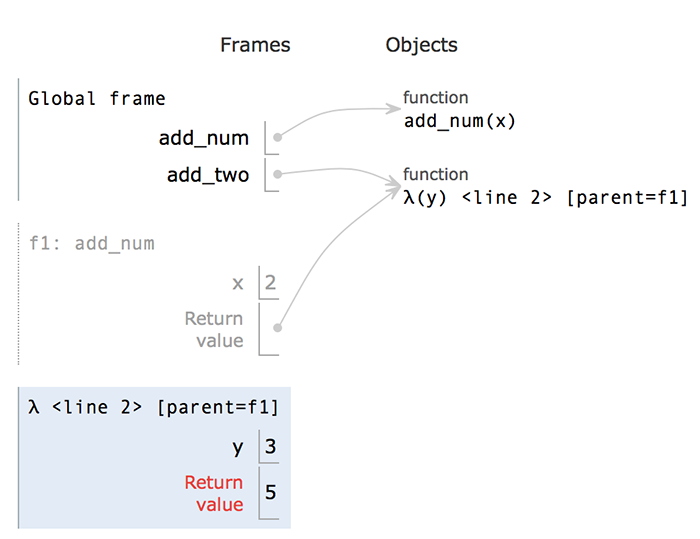
\includegraphics[width=\linewidth]{simple_hof_env.png}
\end{minipage}
Lambdas are represented similiarly to functions in environment diagrams, but
since they lack instrinsic names, the lambda symbol ($\lambda$) is used instead.

\begin{blocksection}
The parent of any function (including lambdas) is always the frame in which the
function is defined. It is useful to include the parent in environment diagrams
in order to find variables that are not defined in the current frame.
In the previous example, when we call \texttt{add\_two} (which is really the
lambda function), we need to know what \texttt{x} is in order to compute
\texttt{x + y}. Since \texttt{x} is not in the frame \texttt{f2}, we look at the
frame's parent, which is \texttt{f1}. There, we find \texttt{x} is bound to
\texttt{2}.

As illustrated above, higher order functions that return a function have their
return value represented with a pointer to the function object.
\end{blocksection}
